\documentclass[11pt]{article}
\usepackage{graphicx,natbib,amsmath,color,matlab-prettifier,listings,epstopdf}
\definecolor{mygreen}{RGB}{28,172,0}
\definecolor{mylilas}{RGB}{170,55,241}
\title{The Portfolio Selection Problem}
\author{Deniz Dilan Dogan}
\begin{document}

	\maketitle
	\tableofcontents
\pagebreak
\section{Introduction}
\subsection{The problem}
This problem is an investor's problem: the tradeoff between risk and return. The risk being that the average return is lower than expected. The return of the portfolio is given by the sum of the product of the fraction of investment in asset $i$ and the expected return of asset $i$. We are able to measure the risk of a portfolio by considering the dispersion of a returns given by a portfolio i.e.the range of its returns, the definition of volatility then follows as the measure of this dispersion. Measures to determine the volatility of a portfolio include the standard deviation which is dispersion relative to average returns, and variance which is the standard deviation squared. When considering a portfolio we must consider the joint variability, which is the variabilty of all assets combined in a given portfolio, to find the associated risk of the portfolio. It is important to acknowledge that, even if average return of a portfolio is the same as another portofolio, the risk defined by this joint variability can significantly change the actual returns. Hence we can form a minimization problem, the objective being to minimize the risk of the portfolio of assets while considering the minimum amount of return the investor desires. This is only one approach to the problem, we can also take the approach of maximizing returns given the maximum amount of risk an investor is willing to take in the form of standard deviation or variance.
\subsection{Potential Constraints}
Constraints of this problem may include: the wealth of the investor, even a wealthy investor has a limit since wealth is finite. Following that constrant, the amount the investor is willing to invest (we can avoid this constraint by giving the portfolio as a fraction of investments into assets). The risk the investor is willing to take i.e. their risk tolerance, when minimizing the risk this 'risk tolerance' can be directly implemented into the objective function, so it is an implied constraint rather than an explicit one. However, when maximizing return this 'risk tolerance' is an explicit constraint considered using the maximum variance. The minimum acceptable return of a portfolio, the portfolio must give returns equal to or greater than this value. The basic non-zero constraints on fractions of investment. Futher constraints can be given by asset types i.e. some assets have a minimum and/or maximum amount of investment. It is clear that most of these constraints are dependent on the investor, hence the problem can be catered to an individual investor by altering constraints in accordance to the investor's desires and risk tolerance.
\subsection{Defining Variables}
{\boldmath$x$}: Vector of fractions of investments in assets $i=1,2,..,n$ where component $x$$_i$ is fraction of investment in asset i.
\newline {\boldmath$\mu$}: Vector of expected returns of assets $i=1,2,...,n$ where component $\mu$$_i$ is the expected return of asset i.
\newline $\mathbf{r}$: Vector of returns of assets $i=1,2,...,n$ where component $v$$_i$ is the return of asset i.
\newline $r$$_i$: The return given by asset i, this is unknown and treated as a random variable that follows a normal distribution.
\newline $\rho$$_{ij}$: Correlation between asset i and asset j.
\newline $\sigma$$_i^2$: Variance associated with asset i.
\newline $G$: Covariance matrix which is a $n$ x $n$ symmetric positive semidefinite matrix where component $G_{ij}=\rho_{ij}\sigma_i\sigma_j$.
\newline  $\mu$$_*$: The minimum acceptable return.
\newline  $\sigma_*^2$: The maximum acceptable variance.
\newline $\lambda_i$: The Lagrange multiplier associated with constraint i of the problem.
\newline $E[R]$: Expected return which is given by $\mathbf{x^T}\boldsymbol\mu$
\newline $Var[R]$: Variance which is given by $\mathbf{x^T}G\mathbf{x}$
\subsection{The Efficient Frontier: a visualisation of the problem}
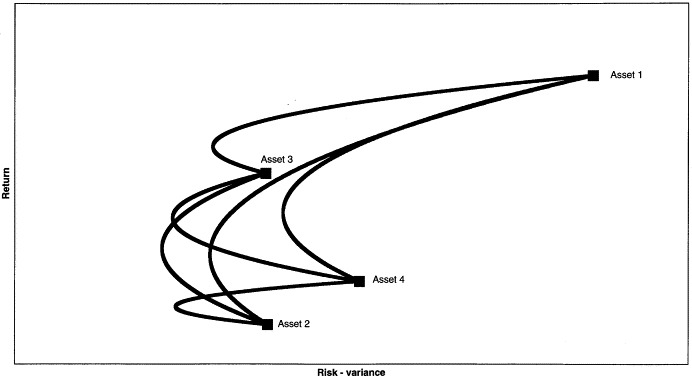
\includegraphics[scale=0.5]{EF} \citep{https://doi.org/10.1111/1540-6229.00689}
\newline Here is an example of an efficient frontier formed by a portfolio of 2 assets. The x-axis represents the risk which is calculated by the joint variability of the assets and the y-axis represents the corresponding return of the portfolio. There are 4 assets at play, changing the fractions of investment between the asset gives the curve between them. Since the curves between all assets are dominated by the curve between asset 1 and asset 3, this curve must contain the efficient frontier since there should be no portfolios above the efficient frontier. Following this idea we can see that investing fully into asset 3 is suboptimal, as from observation we can see there exists a portfolio with the same risk and higher corresponding returns. However fully investing in asset 1 may give the highest expected return, but it also gives the highest risk. The optimal portfolio requires investment of some fraction into both assets to maximize return while reducing the associated risk. Consider tangent line of this curve that is parallel to the y-axis. From observation we can deduct that this tangent point gives the minimum variance portfolio, and all the points up to and including the point of fully investing into asset 1 form the efficient frontier as there are no other portfolios that give lower risk and higher return. Hence this is the line of optimal portfolio selection i.e. the efficient frontier.
\subsection{Modern Portfolio Theory}
Modern portfolio theory was formed to solve the problem described in the subsection 'The Problem'. The key decision that investors must make is how to invest among various assets, this decision is made under great uncertainty hence methods of optimization were desired. The first to clearly formulate and in turn solve the portfolio selection problem was Markowitz. The theory he formed the foundations for is used to tackle how to select a portfolio given a set of assumptions \citep{CONSTANTINIDES19951}
\newline Assumptions are necessary to simplify the portfolio selection problem. Some of these assumptions are about investors such as: assuming that the investor is rational which allows the problem to have an objective function to either minimize risk given minimum acceptable returns or maximize returns given maximum risk investor is willing to take. Some assumptions are about the market for example: that information is symmetric i.e. everyone has equal access to all information relevant to the problem. Futher assumptions are formed when considering how risk behaves, risk aversion is assumed to be linear or constant even though there exists significant evidence that implies the opposite. \citep{doi:10.1080/20430795.2012.738600}
\section{Correlation between assets}
\subsection{Introduction to Correlation}
The correlation between asset $i$ and asset $j$ is the degree of the relationship between their price movements given by
\newline $\rho_{ij}=\frac{E[(r_{i}-\mu_{i})(r_{j}-\mu_{j})]}{\sigma_{i}\sigma_{j}}$  for assets $i,j=1,2,...,n$
\newline Choosing assets such that the correlation between the given assets have the minimum amount of correlation in turn gives minimial risk associated with portfolio with an acceptable return. Going back to defined variables we know that the covariance matrix has elements $G_{ij}$ defined by the product of the correlation between asset $i$ and asset $j$ and the standard deviation of each asset. The covariance matrix is in the objective function when minimizing the risk, further outlining the importance of correlation in this problem.
\subsection{Positive Correlation}
Consider asset $i$ and asset $j$, they have a positive correlation if the assets have the move in the same way. In this case if asset $i$ increases in value, asset $j$ will also increase in value, likewise if asset $j$ increases in value asset $i$ also increases in value. The combination of these assets in a portfolio have a high maximum return however they also have much higher risk. The portfolio selection problem will avoid this case, as it contradicts the assumption that investors are rational, as there is no asset to rely on given the risk becomes a reality. Just by observation of the top assets we can see that Google assets are positively correlated with many other assets including but not limited to: Amazon, Facebook, and Apple assets.
\subsection{Negative Correlation}
Consider asset $i$ and asset $j$, they have a negative correlation if the assets have the move in opposite ways to eachother. If asset $i$ increases in price value, asset $j$ will decrease in price value, likewise if asset $j$ increases in price value asset $i$ decreases  in price value. The combination of these 2 assets give a portfolio of a much lower expected return but in turn a lower risk associated with the portfolio. Hence this portfolio is a good choice to manage risk, even eliminate risk given perfect negative correlation. But it is also suboptimal in terms of return. An example of negative correlation includes: the correlation between airline stocks and oil prices.
\subsection{No Correlation}
Consider asset $i$ and asset $j$, if asset $i$ and asset $j$ show no relationship to each other i.e. using the change in asset $i$ you cannot predict how asset $j$ will change. This is theoretically ideal for a portfolio as it minimizes the risk and has a reasonable minimum return. Gold is known for it's lack of correlation with most other assets. However, most assets are positively correlated so it is hard to select an optimal portfolio.
\section{ Lagrangian Method}
\subsection{Lagrangian Function}
Consider the following problem:
\newline minimize 
$\frac{1}{2} \mathbf{x^T}G\mathbf{x}$
\newline subject to
$\mathbf{x^T}  \boldsymbol\mu \geq \mu_{*}$ and $\sum_{i=1}^{n}  x_{i}=1$ 
\newline In this problem we are minimizing risk which is given by objective function, with consideration of investor's risk tolerance which is implenmented into the objective fuction. Respectively the first constraint is the to ensure $\mathbf{x}$ gives at least the minimum acceptable return given by $\mu_{*}$. The second constraint is to ensure the sum of all fractions of investments gives 1, this simply means that you must invest all the money the investor put forward not just a percentage of it.
\newline The Lagrangian function is given by:
\begin{equation*}
L\left (\mathbf{x},\lambda_{1},\lambda_{2} \right) = \frac{1}{2}  \mathbf{x^T}G\mathbf{x} + \lambda_{1} \left ( \mu_{*} - \mathbf{x^T}  \boldsymbol\mu \right ) + \lambda_{2} \left (1 - \sum_{i=1}^{n}  x_{i} \right) 
\end{equation*}
Consider a portfolio of 3 assets, this gives the following Lagrangian function:
\begin{equation*}
\begin{aligned}
L\left (x_{1},x_{2},x_3,\lambda_{1},\lambda_{2} \right)=&\frac{1}{2}\sum_{i=1}^{3} x_{i}\left(G_{i1}x_{1}+G_{i2}x_{2}+G_{i3}x_3\right) \\
&+ \lambda_{1} \left ( \mu_{*}-\mu_{1}x_{1}-\mu_{2}x_{2}-\mu_3x_3\right) \\
&+\lambda_{2} \left (1-x_{1}-x_{2}-x_3\right) 
\end{aligned}
\end{equation*}
The Lagrangian function is formed by the sum of the objective function, and the product of lagrange multipliers with constraints (hence why we have 3 lagrange multipliers in a 3 constraint problem) which are given in the form of production minus output.
\subsection{First Order Conditions}
In order to derive first order conditions for the 3 asset case, we set the following partial derivatives to 0
\newline $\frac{\partial L}{\partial x_{1}}=0,  \frac{\partial L}{\partial x_{2}}=0, \frac{\partial L}{\partial x_{3}}=0, \frac{\partial L}{\partial \lambda_{1}}=0 , \frac{\partial L}{\partial \lambda_{2}}=0$.
\newline calculating the partial derivatives give
\newline  $\frac{\partial L}{\partial x_{1}}=\frac{1}{2}\left(2G_{11}x_1+\left(G_{12}+G_{21}\right)x_{2}+\left(G_{13}+G_{31}\right)x_{3}\right)+\lambda_1\mu_1-\lambda_2$,
\newline  $\frac{\partial L}{\partial x_{2}}=\frac{1}{2}\left(2G_{22}x_2+\left(G_{21}+G_{12}\right)x_{1}+\left(G_{23}+G_{32}\right)x_{3}\right)+\lambda_1\mu_2-\lambda_2$,
\newline  $\frac{\partial L}{\partial x_{3}}=\frac{1}{2}\left(2G_{33}x_3+\left(G_{31}+G_{13}\right)x_{1}+\left(G_{32}+G_{23}\right)x_{2}\right)+\lambda_1\mu_3-\lambda_2$,
\newline  $\frac{\partial L}{\partial \lambda_{1}}=\mu_{*}-\mu_{1}x_{1}-\mu_{2}x_{2}-\mu_3x_3 $,
\newline $\frac{\partial L}{\partial \lambda_{2}}=1-x_1-x_2-x_3$,
\newline Hence the first order conditions are given by the system of 5 equations
\newline $\frac{1}{2}\left(2G_{11}x_1+\left(G_{12}+G_{21}\right)x_{2}+\left(G_{13}+G_{31}\right)x_{3}\right)+\lambda_1\mu_1-\lambda_2-\lambda_3=0$,
\newline $\frac{1}{2}\left(2G_{22}x_2+\left(G_{21}+G_{12}\right)x_{1}+\left(G_{23}+G_{32}\right)x_{3}\right)+\lambda_1\mu_2-\lambda_2-\lambda_3=0$,
\newline $\frac{1}{2}\left(2G_{33}x_3+\left(G_{31}+G_{13}\right)x_{1}+\left(G_{32}+G_{23}\right)x_{2}\right)+\lambda_1\mu_3-\lambda_2-\lambda_3=0$,
\newline $\mu_{*}-\mu_{1}x_{1}-\mu_{2}x_{2}-\mu_3x_3=0$,
\newline $1-x_1-x_2-x_3=0$.
\subsection{Minimum acceptable returns and minimum variance}
Suppose there exist 3 assets $i=1,2,3$. Each asset has variance of 1 which gives $\sigma$$_i^2=1$ for all assets $i=1,2,3$. The assets are uncorrelated hence $\rho$$_{ij}=0$ for all combinations of assets $i,j=1,2,3$ which means all elements in the covariance matrix are $G_{ij}=0$ which implies Var[R]=0. Hence the minimum variance is given by $\sigma_*=0$. The expected returns of assets are given by $\mu_{1}=1$, $\mu_{2}=2$ and $\mu_{3}=3$ and the fractions of investments must still satisfy $\sum_{i=1}^{n}  x_{i}=1$, there are no constraints for variance as $Var[R]=0$ for all fractions of investments. This further outlines the why uncorrelated assets are optimal, as a portfolio of uncorrelated assets has less constraints. Since the returns are given by $\mathbf{x^T}\boldsymbol\mu $, the minimum return must be given by the following minimization problem:
\newline Minimize $x_1+2x_2+3x_3$ 
\newline subject to $x_1+x_2+x_3=1$ and $\mathbf{x} \geq \mathbf{0}$
\newline to solve this linear programming problem I used inbuilt MATLAB Optimization Toolbox\citep{MATLAB1} the minimum returns are given when $x_1=1$, $x_2=0$ and $x_3=0$ plugging these values into  $\mathbf{x^T}\boldsymbol\mu $ gives minimum return $\mu_*=1$. 
\section{Example}
\subsection{Problem}
Minimize
$\frac{1}{2} \mathbf{x^T}G\mathbf{x}$
\newline subject to
$\mathbf{x^T}  \boldsymbol\mu = 0.11$ , $\sum_{i=1}^{3}  x_{i}=1$
\newline where, 
\begin{equation*}
G=
\begin{pmatrix} 
0.00015 & 0.00005 & -0.00007\\
0.00005 & 0.00025 & -0.00003\\
-0.00007 & -0.00003 & 0.00010
\end{pmatrix}
\end{equation*}
and
\begin{equation*}
\boldsymbol\mu=
\begin{bmatrix} 
0.11\\
0.15\\
0.08
\end{bmatrix}
\end{equation*}

\subsection{Solution}
Since $x_{i}$ is the fraction of investment into asset $i$ the solutions are given by $x_{1}=\frac{202}{615}$, $x_{2}=\frac{59}{205}$ and $x_{3}=\frac{236}{615}$ with an associated variance given by $Var[R]=0.00003679675$ and return given by $E[R]=0.11$ which is given by the constraint $\mathbf{x^T}  \boldsymbol\mu = 0.11$. 
\newline 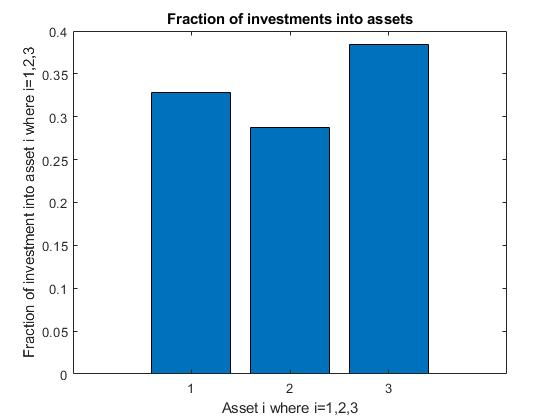
\includegraphics[scale=0.6]{PSPfig1} 
\section{Other methods}
\subsection{Quadratic Programming}
Quadratic programming solves problems with a quadratic objective function, lets apply this inbuillt MATLAB code\citep{MATLAB2} to the problem in section 4.1 to compare the solutions found from my code in section 4.2. $x_{1}=0.0328459$, $x_{2}=0.2878033$ and $x_{3}=0.3837377$ with an associated variance given by $Var[R]=0.00003679675$ and return given by $E[R]=0.11$ which is given by the constraint $\mathbf{x^T}  \boldsymbol\mu = 0.11$. This is equivalent to my solutions in section 4.2, this is because both methods use the same Lagrangian approach but the quadratic programming method takes a mere $0.0282923seconds$ to give solutions whereas my code is computationally expensive hence takes significantly more time to find solutions. This method also is more flexible i.e. can be applied to a wider range of problems with more than 3 assets in play. My code is specifically made for 3 assets, for more than 3, I would have to add to my code and change some parts for example, the $\mathbf{x}$ matrix. Most importantly we can apply large data sets to quadratic programming.
 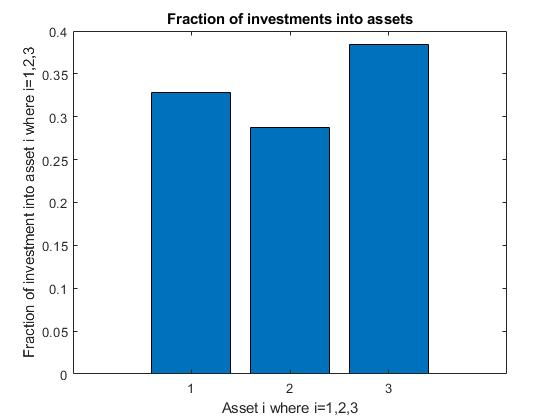
\includegraphics[scale=0.6]{PSPfig2} 
\newpage
\bibliography{OFEbib}
\bibliographystyle{unsrt}
\newpage 
\section{Appendices}
\lstinputlisting[style=Matlab-editor,caption={Finding minimum return using Optimization Toolbox on MATLAB corresponding to section 3.3} ]{PSP2.m}
\begin{verbatim}
investing a fraction of 1 into asset 1, a fraction of 0 into asset 2 
and a fraction of 0 into asset 3 gives minimum return 1
\end{verbatim}
\lstinputlisting[style=Matlab-editor,caption={Solution given by the Lagrangian method of optimization on MATLAB corresponding to section 4.2} ]{PSP.m}
\begin{verbatim}
invest a fraction of 202/615 into asset 1, invest a fraction of 
59/205 into asset 2, invest a fraction of 236/615 into asset 3
and the associated variance of this portfolio is given by 3.679675e-05
\end{verbatim}
\lstinputlisting[style=Matlab-editor,caption={Solution given by the Quadratic programming on MATLAB corresponding to section 5.1} ]{PSP3.m}
\begin{verbatim}
Solving problem using quadprog.

 Iter            Fval  Primal Infeas    Dual Infeas  Complementarity  
    0    6.050000e-05   6.500000e-01   4.325038e-01     1.666667e-01  
    1    1.840942e-05   1.387779e-17   5.551115e-17     2.529345e-02  
    2    1.840942e-05   1.110223e-16   3.697129e-17     1.272311e-05  
    3    1.840342e-05   0.000000e+00   8.809143e-20     7.746379e-08  
    4    1.839837e-05   0.000000e+00   1.355253e-20     5.002860e-11  

Minimum found that satisfies the constraints.

Optimization completed because the objective function is non-decreasing in 
feasible directions, to within the value of the optimality tolerance,
and constraints are satisfied to within the value of the constraint tolerance.

Elapsed time is 0.028923 seconds.
invest a fraction of 3.284590e-01 into asset 1, invest a fraction of 2.878033e-01
into asset 1, invest a fraction of 3.837377e-01 into asset 3 with an associated
variance 3.679675e-05
\end{verbatim}


\end{document}